\section{Comparing StableMoor $\ulow$ to IMU $\uhead$}
\label{apdx:ulow}

It is instructive to compute compare the motion of the StableMoor buoy as measured by the Compare the motion correction of SM to TTM: SM does better because it is more stable, and has a measurement of $u_\mathrm{low}$. Discuss spectral coherence of $u_\mathrm{BT}$ with IMU, i.e. Figure \ref{fig:SM_coh}. This is important because it shows the low-$f$ limit of the IMU measured motion.

\begin{figure}[t]
  \centering
  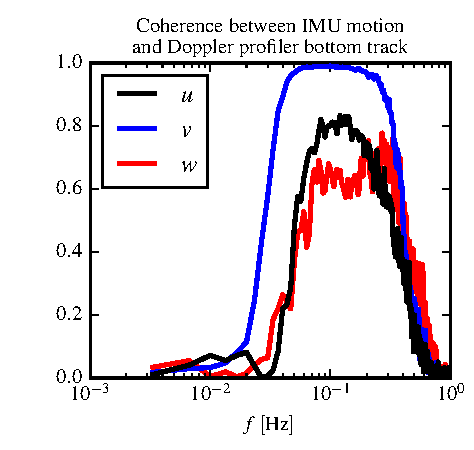
\includegraphics{BT_IMU_Coherence02}
  \caption{Coherence between stablemoor IMU measured motion and bottom track velocity.}
  \label{fig:SM_coh}
\end{figure}



%%% Local Variables:
%%% mode: latex
%%% TeX-master: "Kilcher_etal_IMU-ADV"
%%% End:
